\chapter{Statistical Mechanical Ensembles and Potential Energy Surfaces} \label{ch:pes_e}
\section{Introduction}
The approach taken in this work for solving the atomic structures of materials is one of optimization.
The plan is to develop a potential energy surface (PES) which has minima associated with atomic structures who's properties match the experimentally observed properties.
Thus, the various positional variables of the structure can be solved by optimizing the structure against the PES.
This approach is popular in the PDF community for solving the structure of materials using both extensive large box models and simpler small box models.

In this chapter we discuss the development of the various PESs used in the PDF community for comparing theoretical and experimental PDFs.
Special attention will be paid to the gradients of the potential energy functions, as these are important to some optimization techniques.
Additionally, we also discuss the use of statistical mechanical ensembles for finding minima on the PES.

\section{Potential Energy Surfaces} \label{sec:pes}
A PES simply describes the potential energy of the system as a function of all its relevent coordinates in phase space, essentially providing a mapping $\mathbb{R}^{n} \rightarrow \mathbb{R}$, where $\mathbb{R}$ is the set of real numbers and $n$ is the number of positional parameters in the system.
Usually these coordinates are the positions of the atoms $q$ and their conjugate the momenta $p$.
Note that there could be more variables associated with the system, for instance the magnetic moments of the atoms could play a role in describing the system.
In this magnetic system there would be positional variables for the atomwise spin vectors and their "momenta".
Application of the term "momenta" might seem odd here, as the magnetic spin does not have a mass or a velocity.
However, since the magnetic "position" is defined on the PES we need to describe its conjugate varible to properly formulate Hamitonian dynamics and the kinetic portion of the PES.

\subsection{Experimentally Derived Potential Energy Surfaces}
Generally PESs are obtained from purely computational experiments including: ab-initio DFT, classical approximations via the embedded atom method, or even parameter driven models with experimentally fitted parameters.
However, one can dervive a PES from an experiment which describes how well the model reproduces the experimental data.
In this case one needs a theoretical and computational framework mapping the atomistic variables of the simulation to the same space of the data obtained from the experiment.
This allows the experiment to be compared directly against the predicted data via an experimentally derived PES.
\subsubsection{Potentials}
For an experiment which produces 1D data, like powder diffraction, EXAFS or XPS, the implemented potentials are:
\begin{equation} \label{chi}
\chi^{2} =
\sum_{a=a_\mathrm{min}}^{a_\mathrm{max}} \left(A_{_\mathrm{obs}} - \alpha A_{_\mathrm{calc}}\right)^{2}
\end{equation}
\begin{equation}\label{Rw}
Rw =
\sqrt{\frac{\sum_{a=a_\mathrm{min}}^{a_\mathrm{max}} \left(A_{_\mathrm{obs}} - \alpha A_{_\mathrm{calc}}\right)^{2}}{\sum_{a=a_\mathrm{min}}^{a_\mathrm{max}} A_{_\mathrm{obs}}^{2}}}
\end{equation}
\begin{equation}\label{INVERT}
  \chi^{2}_{\mathrm{INVERT}} = \frac{1}{N}\sum_{j}\sum_{r}[A_{obs}(r) - \alpha A_{j_\mathrm{calc}}(r)]^{2}
\end{equation}
\begin{equation} \label{alpha}
\alpha  = \frac{\sum_{a=a_\mathrm{min}}^{a_\mathrm{max}}A_\mathrm{_\mathrm{obs}}A_{_\mathrm{calc}}}{\sum_{a=a_\mathrm{min}}^{a_\mathrm{max}} A_{_\mathrm{calc}}^{2}} = \frac{\vec{A}_{_\mathrm{obs}}\cdot\vec{A}_\mathrm{calc}}{|\vec{A}_\mathrm{calc}|^{2}}
\end{equation}
where $A_{calc}$ and $A_{obs}$ are the calculated and observed 1D experimental data
and $A_{calc, j}$ is the calculated data for a single atom interacting with the other atoms of the system.
Note that $A_{calc}$ has a dependence on $q$, the positions of the system.

The $Rw$ and $\chi^{2}$ potentials have been reported numerous times. \cite{Petkov2014, Masadeh2007, Choi2013, McGreevy, Proffen1997}
Essentially these potentials measure the least squares distance between the observed scattering and the predicted scattering poviding a way to quantify the agreement between the model and experiment.
While $RW$ and $\chi^{2}$ are now standard in the PDF community, the $\mathrm{INVERT}$ potential is fairly new and aims to incorperate descriptions of the structural symmetry into the PES. \cite{Cliffe2010, Cliffe2013}
In the case of the $\mathrm{INVERT}$ potential NMR or other symmetry sensitive data is used to describe the number of unique atomic coordinations.
This is then used to describe the number of unique atomwise pair distribution functions, thus causing systems with more or less unique coordination environments to be higher in energy.
This approach has been shown to be useful for \ce{C60} and other systems which are highly symmetric, creating a PES with an easier to find minima. \cite{Cliffe2010, Cliffe2013}
However, many times this kind of data is unavailable when refining the structure causing the potential to be less useful.
Additionally, this potential introduces an element of user bias as the refiner must decide, based on some spectroscopic data, how many unique environments are in the material.
This bias could be removed by using one of the other potentials with a method for simulating the observed spectra, allowing the computational system decide what structures properly reproduce all the observed data.

\subsubsection{Forces}
\begin{equation}
\grad{\chi^{2}} =
- 2 \sum_{a=a_\mathrm{min}}^{a_\mathrm{max}} (\alpha \frac{\partial A_{_\mathrm{calc}}}{\partial \gamma_{i, w}} + A_{_\mathrm{calc}} \frac{\partial \alpha}{\partial \gamma_{i, w}} ) (A_{_\mathrm{obs}} - \alpha A_{_\mathrm{calc}})
\end{equation}
\begin{equation}
\grad{Rw} =
\frac{Rw}{\chi^{2}} \sum_{a=a_\mathrm{min}}^{a_\mathrm{max}} (\alpha \frac{\partial A_{_\mathrm{calc}}}{\partial \gamma_{i, w}} + A_{_\mathrm{calc}} \frac{\partial \alpha}{\partial \gamma_{i, w}} ) (\alpha A_{_\mathrm{calc}}  - (A_{_\mathrm{obs}}))
\end{equation}
\begin{equation}
  \grad{\chi^{2}_{\mathrm{INVERT}}} = \frac{-2}{N} \sum_{a=a_\mathrm{min}}^{a_\mathrm{max}} \sum_{j}(\alpha \frac{\partial A_{j_\mathrm{calc}}}{\partial \gamma_{i, w}} + A_{j_\mathrm{calc}} \frac{\partial \alpha}{\partial \gamma_{i, w}} ) (A_{_\mathrm{obs}} - \alpha A_{j_\mathrm{calc}})
\end{equation}
\begin{equation}
\frac{\partial \alpha}{\partial \gamma_{i, w}}  =
\frac{(\sum_{a=a_\mathrm{min}}^{a_\mathrm{max}} A_{_\mathrm{obs}} \frac{\partial A_{_\mathrm{calc}}}{\partial \gamma_{i, w}}- 2\alpha \sum_{a=a_\mathrm{min}}^{a_\mathrm{max}} A_{_\mathrm{calc}} \frac{\partial A_{_\mathrm{calc}}}{\partial \gamma_{i, w}})}{\sum_{a=a_\mathrm{min}}^{a_\mathrm{max}} A_{_\mathrm{calc}}^{2}}
\end{equation}
where $\gamma_{i, w}$ is the $i$th arbitrary positional variable in the $w$th direction.
The concept of an "arbitrary positional variable" might seem a bit cumbersome but it allows us to define the forces for any atomic parameter which can be represented as a vector in 3-space.
This comes in handy when trying to define the forces acting on variables like anistropic displacement parameters or atomic magnetic spins.

\graphicspath{{./pes_e/figures/}}
\section{Ensembles} \label{sec:ens}
While PESs describe which atomic configurations are the most desirable and how the atoms would like to get there, the ensemble describes how the atoms move on the PES.
The abstraction of the PES from the ensemble is an important one, as it allows for the reuse and exchange of both PESs and ensembles for a wide array of problems.
Statistical mechanical ensembles can be described in two ways, analytically and scholastically.
For long simulation times and fine enough numerical or analytical integration these two descriptions should be identical.

In either case one starts by defining the Hamiltonian, $\mathcal{H}$, as the total energy of the system.
Thus, the Hamiltonian is described as the sum of the potential $U(q)$ and kinetic $K(p)$ energies, where $q$ is the positions of the atoms and $p$ is their momenta
\begin{equation} \label{Hamiltonian}
  \mathcal{H}(q, p) = U(q) + K(p)
\end{equation}
\noindent where $K(p) = \frac{1}{2}\sum_{i} \frac{p_{i}^{2}}{m_{i}}$ and $i$ denotes the $i$th particle.

Analytically one generally defines a partition function, which describes the sum of probabilities over all potential atomic states.
\begin{equation}
\Xi = \sum_{i} P_{i}(q, p)
\end{equation}
where $P_{i}$ is the probability of the $i$th state and is a function of the total energy of that state.
This partition function can then be used to obtain the probability of any specific state.
The relationship of the probability of a state to the state's energy and other properties depends on the ensemble being used.
%\begin{equation}
%P(q, p) = \frac{\delta(E - \mathcal{H}(q, p))}{W}
%\end{equation}
%where $E$ is the energy of the system, W is the total number of states in the system, and $\delta$ is the Dirac Delta Function.

For the canonical ensemble the partition function is probability is:
\begin{equation}
Q(N, V, T) = \exp(\frac{-\mathcal{H}(q, p)}{k_{b}T})
\end{equation}
where $k_{b}$ is the Boltzmann constant and $T$ is the temperature of the system. \cite{McQuarrie2000}

\subsection{Monte Carlo Modeling}
Monte Carlo can be used to simulate a statistical mechanical ensemble which can not be solved analytically.
In most Monte Carlo systems the ensemble is simulated by randomly changing one of the system parameters and comparing the energy of the new system against the energy of the old system.
If the energy of the new system is lower than the current energy then the new configuration is accepted.
Otherwise the new system is rejected unless
\begin{equation}
\exp(\frac{-\Delta E}{E_{T}}) < u
\end{equation}
where u is a random number $[0, 1)$ and $E_{T}$ is the thermal energy characteristic to the system.
The ability of Monte Carlo modeling to accept ``bad'' moves allows the system to hop out of local energy minima during the search for the global minimum.
Reverse Monte Carlo (RMC) is similar to Monte Carlo except it uses $\chi^{2}$ as the PES.\cite{McGreevy}

Despite the utility of RMC, and its wide use in the x-ray scattering community, as Hoffman and Gelman state ``Not all MCMC [Markov Chain Monte Carlo] algorithms are created equal''.\cite{Hoffman2014}
RMC, similar to standard Monte Carlo simulations, samples from the PES at random, usually by translating atoms in the system randomly.
This creates a less efficient, random walk based, exploration of the PES.\cite{Hoffman2014, Neal1993}
Thus, methods for suppressing this random walk nature, while still searching the potential energy surface fully are needed.

\subsection{Hamiltonian Monte Carlo}
Hybrid or Hamiltonian Monte Carlo (HMC) can help to address some of these issues.
HMC was developed originally in the lattice quantum chromodynamics community and provides a more efficient, more scalable approach to PES sampling for Monte Carlo.\cite{Duane1987216, Neal2011}
In HMC the PES is explored using Hamiltonian dynamics, essentially following the gradient of the PES to find more acceptable configurations.


In order to model dynamics we need to describe the motion of the particles in our system, thus:
\begin{align}
  \frac{d q_{i}}{d t} &= \frac{\partial \mathcal{H}}{\partial p_{i}} = p_{i}\\
  \frac{d p_{i}}{d t} &= -\frac{\partial \mathcal{H}}{\partial q_{i}} = -\grad{U}
\end{align}
Using these equations we can derive the position and momentum vectors at any point in time using the leap-frog algorithm:
\begin{align}
  p_{i}(t + \delta t/2) &= p_{i}(t) - \frac{\delta t}{2} \frac{\partial }{\partial q_{i}}U(q(t))\\
  q_{i}(t+\delta t)  &= q_{i}(t) + \delta t * p_{i}(t+\delta t/2)\\
  p_{i}(t+\delta t) &=   p_{i}(t + \delta t/2)- \frac{\delta t}{2} \frac{\partial }{\partial q_{i}}U(q(t+\delta t))
\end{align}
Note that $\frac{\partial}{\partial q_{i}}$ is the gradient with respect to $q$ where $i$ denotes the $i$th atom being moved.
Using this notation the gradient is
\begin{equation} \label{grad}
  \grad{U} = \begin{bmatrix}
    \frac{\partial U}{\partial q_{0, x}} & \frac{\partial U}{\partial q_{0, y}} & \frac{\partial U}{\partial q_{0, z}} \\
    \vdots & \frac{\partial U}{\partial q_{i, w}} & \vdots \\
    \frac{\partial U}{\partial q_{n, x}} & \frac{\partial U}{\partial q_{n, y}} & \frac{\partial U}{\partial q_{n, z}} \\
  \end{bmatrix} =
  \begin{bmatrix}
    \vec{\mathcal{F}}_{0} \\
    \vdots \\
    \vec{\mathcal{F}}_{i} \\
    \vdots \\
    \vec{\mathcal{F}}_{n}\\
  \end{bmatrix}
\end{equation}
where $\frac{\partial}{\partial q_{i, w}}$ is the derivative with respect to $q$ where $w$ denotes direction of the derivative ($x$, $y$, or $z$),  $n$ is the number of atoms and $U$ is the potential which depends on $q$, and $\vec{\mathcal{F}_{i}}$ is the "force" on the $i$th atom.
Using these equations new potential configurations are proposed from the PES.
These proposals are checked against the standard Metropolis criteria discussed above, except that the change in potential energy $\Delta E$ is replaced with the change in the Hamiltonian $\Delta \mathcal{H}$.
Note that while this sampling closely simulates the canonical ensemble, it is not exactly the same.
Usually the canonical ensemble is formulated as microcanonical ensembles in contact with an infinite heat bath at a given temperature, or a set of microcanonical ensembles which exchange thermal energy.
However, the HMC ensemble presented here has a momentum bath instead of a temperature bath.
One could imagine the atoms sitting in a simulation box which has walls which can toggle their thermal exchange.
Initially the box starts in the momentum bath, allowing the atoms to come to equilibrium with the bath momentum.
The box is then removed from the bath causing it to become adiabatic.
Hamiltonian dynamics are then propagated inside the box, essentially running a microcanonical simulation.
Once the dynamics are finished the energy of the system is checked with the Metropolis criteria and the box is reintroduced to the momentum bath and the process starts again.

\subsubsection{No-U-Turn Sampling}
Two parameters must be specified in HMC simulations, the step size $\delta$ and the number of steps $N$.
The step size is critical to the stability of the fitting procedure:  with a too small $\delta$ the simulation runs inefficiently producing structures too close to the previous, whereas with a too big $\delta$ the linear approximation for the forces breaks down and often the simulated NP explodes.
The number of steps to take during the dynamics is equally important and an inappropriate choice may result in backtracking or random walk characteristics in the simulations.
In this work, we employ the No-U-Turn Sampling (NUTS) method recently proposed by Hoffman and Gelman to address this issue \cite{Hoffman2014}.
In the NUTS method $\delta$ and $N$ are dynamically computed by examining the ratio of accepted to rejected configurations as well as whether or not the simulation has started to take a U-turn.
The U-Turn criteria makes certain that the simulation stops when it begins to backtrack, preventing excess computation on configurations that have very little new information to offer.
The use of NUTS leaves us with two simulation parameters: the simulation temperature and the target acceptance.
Hoffman and  Gelman have empirically shown that the ideal target acceptance, which governs the dynamics time steps, is .65, which we have used for all of the simulations here.
The simulation temperature sets the magnitude of the random starting momenta for the atoms at the beginning of each dynamics run \cite{Hoffman2014}.

\subsection{Grand Canonical Ensemble}
While NUTS-HMC simulations provide a system to find minima on PESs, the simulation is fundamentally run in the Canonical Ensemble thus the variables in the simulation are limited to a fixed number of particles, simulation volume, and thermal energy.
Fixing the thermal energy and simulation volume is not a problem, as they are not variables of interest in the final structure.
However, specifying the number of atoms in the system can be problematic, as the exact number of atoms in a sample can be difficult to count or a sample could have a distribution of particle sizes.
Thus, a new ensemble needs to be used to allow the number of atoms to vary as a function of the PES.
This new ensemble is the Grand Canonical Ensemble.

\subsubsection{Ensemble description}
In the Grand Canonical Ensemble (GCE) two sets of variables are allowed to change, the atomic positions, and the total number of atoms and their associated identities.
These two variables are controlled by temperature, or average momentum, and chemical potential.
The partition function is
\begin{equation}
  \Xi = \sum_{N=0}^{\infty} Q(N, V, T) \exp{\frac{N\mu\beta}{T}}
\end{equation}
where $Q(N, V, T)$ is the Canonical partition function discussed above, $\mu$ is the chemical potential. \cite{McQuarrie2000}
This is translated into a Monte Carlo system, producing Grand Canonical Monte Carlo (GCMC).
\subsubsection{Grand Canonical Monte Carlo}
While the probabilities for atomic motion are the same as in the Canonical Ensemble, the addition or removal of an atom have their own probabilities. For the addition of an atom the probability is formally:
\begin{equation}
  \min[1, \frac{V}{(N+1) \Lambda(T)^{3}}e^{-\beta\Delta U + \beta \mu}]
\end{equation}
Similarly the removal of an atom has the probability:
\begin{equation}
  \min[1, \frac{(N)\Lambda(T)^{3}}{V}e^{-\beta\Delta U - \beta \mu}]
\end{equation}
However, both of these equations depend of the overall simulation volume and the thermal wavelength, which is undesirable as these are not really properties that we are of interest to these simulations.
Thus, we roll them into the definition of the chemical potential, essentially setting the base chemical potential to counteract these effects.
This makes certain that our simulation does not change if we change the overall cell volume.
A GCMC move consists of creating a new atomic configuration, where an atom has been added or removed, and checking the above criteria.
However, previous results have shown that this method is computationally expensive in dense liquids, and exceedingly expensive in solid materials.
The long simulation times are due to the random nature of the atomic additions or removals which produce: over-tightly packed atoms, atoms in the middle of nowhere, or nonphysical vacancies.
These configurations are rejected by the GCMC criteria but their probability of being sampled is much higher than configurations which are lower in energy, since the number of incorrect ways to add/remove atoms is much larger than the correct ways.
Thus, we have implemented methods for biasing the atomic addition positions and the atomic removals toward configurations which are more likely to be accepted.

\subsubsection{GCMC biasing}
The basic idea of GCMC biasing is mapping, in 3 dimensions, where an atomic addition or removal is most likely to be accepted.
Thus, the simulation volume is broken up into voxels, 3 dimensional volumes which are contained by the total simulation volume, with a pre-set size.
Each voxel is given a probability of being chosen for a trial insertion where the probability is:
\begin{equation}
  P_{i, j, k} = \frac{e^{\beta \Delta U_{i, j, k}}}{\sum_{i, j, k}e^{\beta \Delta U_{i, j, k}}}
\end{equation}
where $\Delta U_{i, j, k}$ is the change in energy.
However, calculating $\Delta U_{i, j, k}$ can be particularly expensive, especially when calculating scattering from atomic positions.
The computational expense can be mitigated by using a cheaper potential, if only for the evaluation of the voxel energy, as previously shown.
Similar to previous work we can use the Lennard Jones potential to approximate the addition potential, lowering the computational burden. \cite{Snurr1993}

Atomic deletion follows a similar biasing procedure, calculating the energy of each atom and biasing the probability of each atom to be chosen for removal by its energy.
This way atoms which add the most energy to the system are more likely to be removed.

\begin{figure}
    \centering
    \subfloat[]{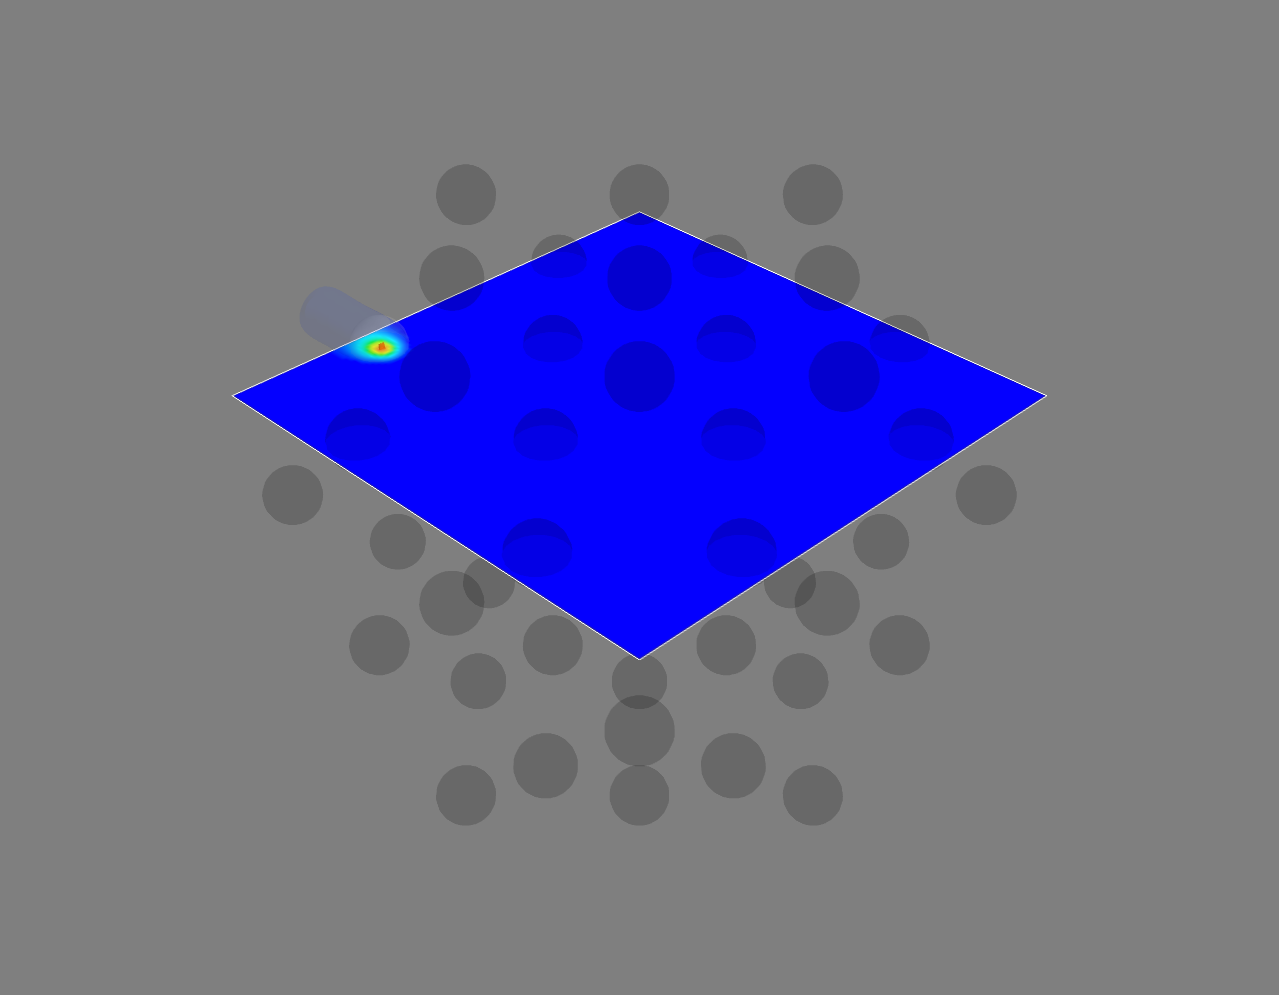
\includegraphics[width=.8\textwidth]{snapshot}\label{subfig: biasing_map}} \\
    \subfloat[]{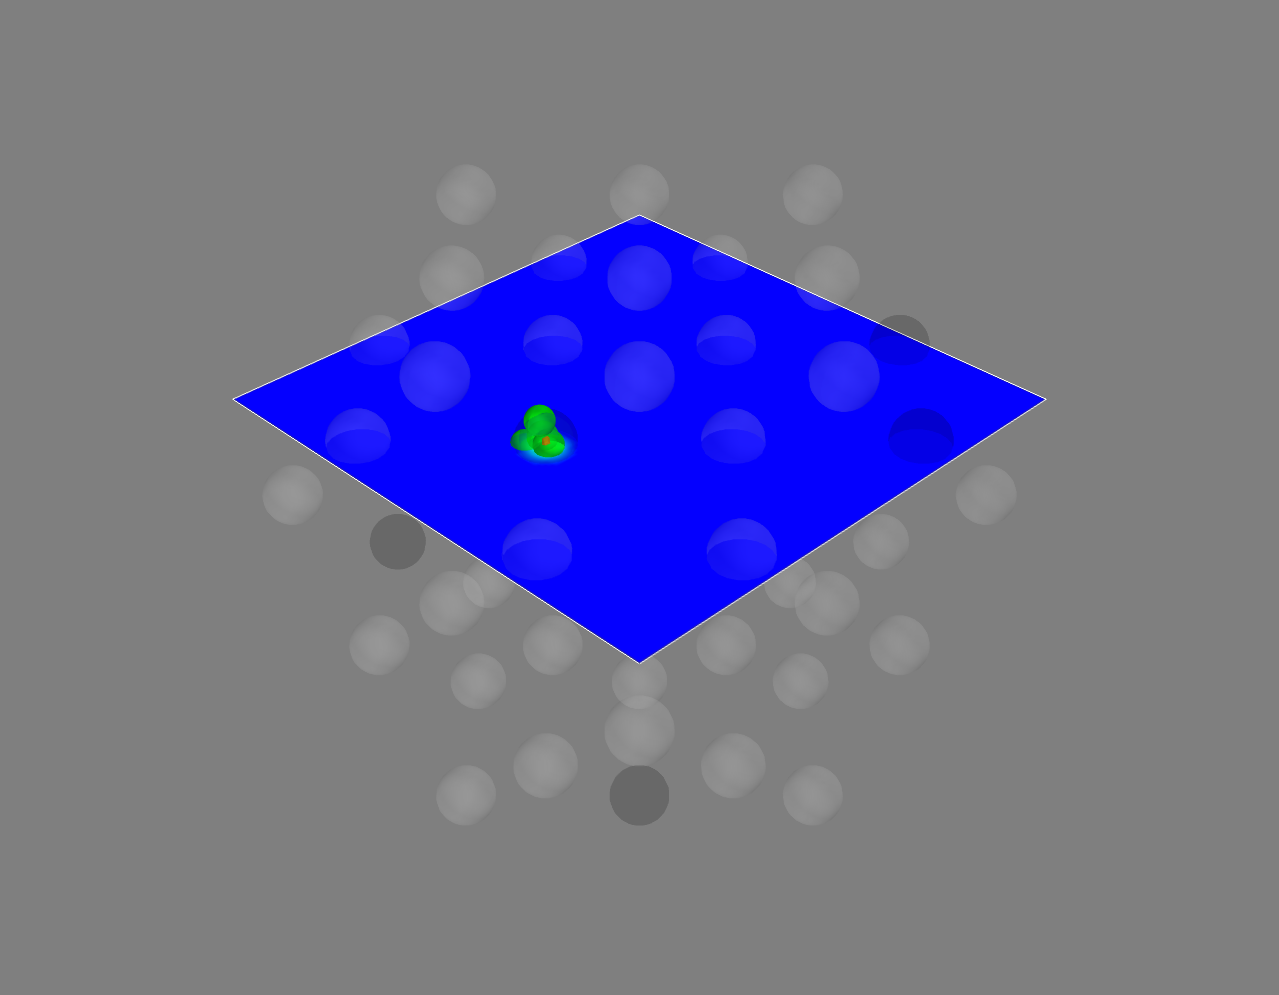
\includegraphics[width=.8\textwidth]{gc_positioning_snapshot}\label{subfig: insertian_trials}}
	\caption[Addition biasing with a Lennard Jones potential.]{These figures show slices of the three dimensional addition potential energy surface. a) shows the addition probability, with the red area most probable. b) shows the results of trial insertions, where the green spheres denote where insertions were attempted.}
	\label{fig:biasing}
\end{figure}
Figure \ref{subfig: biasing_map} shows an example map for atomic addition in a Au54 atom system, with an Au55 atom target.
Figure \ref{subfig: insertian_trials} shows the results of a few GCMC insertions with biasing, showing the focusing of the simulation on the missing atom.
The high density of insertions around the missing atom would not have been possible without the biasing.


\section{Conclusions}
In this chapter we have presented the development of both PES and the statistical mechanical ensembles used to search them.
We expanded the classical concept of a PES to a more generall mapping from positional variable space to energy space.
This expantion allowed for the implementation of experimentally derived PES, where the disagreement between experimental and computed results can be included in the PES.
Common experimental PESs were discussed, and their forces derived.
The implementation of various statistical mechanical ensembles, used for searching the PES for minima, was also discussed with a special focus on No-U-Turn-Sampling Hamiltonian Monte Carlo.
Grand Canonical Monte Carlo was also discussed, with an emphasis on the us of biasing to increase the overall acceptance rate.
Future work in this area may include the development of PESs which leverage 2 dimensional data, like STEM images, or ensembles which help to eliminate tuned parameters like parallel tempering.
